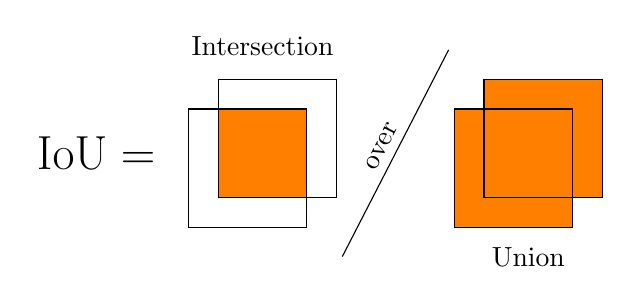
\begin{tikzpicture}[scale=0.75]
  \node[left] at (-0.4, 1.25) {\LARGE $\mathrm{IoU} = $};
  % Intersection illustration
  \begin{scope}
    \clip (0, 0) rectangle (2, 2);
    \fill[orange] (0.5, 0.5) rectangle (2.5, 2.5);
  \end{scope}
  \draw (0, 0) rectangle (2, 2);
  \draw (0.5, 0.5) rectangle (2.5, 2.5);
  \node[above, yshift=0.5em] at (1.25, 2.5) {Intersection};

  % Division sign
  \draw (2.6, -0.5) -- node[auto, sloped] {over} (4.4, 3);

  % Union illustration
  \begin{scope}[shift={(4.5, 0)}]
    \draw[fill=orange] (0, 0) rectangle (2, 2);
    \draw[fill=orange] (0.5, 0.5) rectangle (2.5, 2.5);
    \draw (0, 0) rectangle (2, 2);
    \node[below, yshift=-0.4em] at (1.25, 0) {Union};
  \end{scope}
\end{tikzpicture}
